\documentclass[12pt]{article}
\usepackage{../../ficha}

\begin{document}

\ficha{Conjuntos e Diagramas de Venn}

\instrucoes{Resolve os exercícios. $A \cup B$ é a reunião, $A \cap B$ a interseção, $\overline{A}$ o complementar e $A \setminus B$ a diferença.}

\secao{Definir Conjuntos}{Define cada conjunto em extensão (enumerando os elementos).}
\begin{exercicios}
  \item $A$ = conjunto das vogais.
  \item $B$ = conjunto dos números naturais menores do que 7.
  \item $C$ = conjunto dos números pares entre 10 e 20.
  \item $D$ = conjunto dos divisores de 12.
  \item $E = \{x \in \N : x^2 < 30\}$.
  \item $F = \{x \in \Z : -2 \le x < 3\}$.
  \item Completa com $\in$ ou $\notin$: $\;5 \;\square\; B$, $\;12 \;\square\; C$, $\;6 \;\square\; D$, $\;0 \;\square\; F$.
  \item Indica o cardinal de cada um dos conjuntos anteriores.
  \item O conjunto dos números naturais pares e ímpares ao mesmo tempo tem quantos elementos? Como se chama?
\end{exercicios}

\secao{Operações com Conjuntos}{Considera $U = \{1, 2, 3, 4, 5, 6, 7, 8, 9, 10\}$, $A = \{1, 2, 3, 4, 5\}$, $B = \{2, 4, 6, 8, 10\}$ e $C = \{3, 6, 9\}$. Determina:}
\begin{exercicios}
  \item $A \cup B$
  \item $A \cap B$
  \item $B \cap C$
  \item $A \cap C$
  \item $\overline{A}$
  \item $\overline{B}$
  \item $A \setminus B$
  \item $B \setminus A$
  \item $(A \cup B) \cap C$
  \item $\overline{A \cup B}$
  \item $A \cap B \cap C$
  \item Representa $A$, $B$ e $C$ num diagrama de Venn.
\end{exercicios}

\secao{Ler Diagramas de Venn}{Observa o diagrama de Venn e responde.}

\begin{center}
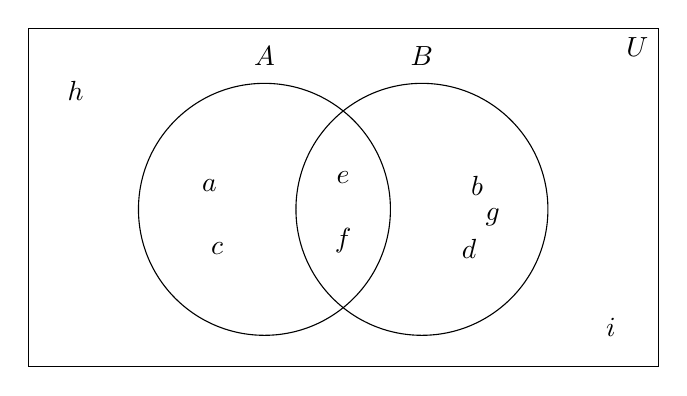
\begin{tikzpicture}
  \draw (-3,-2) rectangle (5,2.3) node[below left] {$U$};
  \draw (0,0) circle (1.6) node[above=1.7cm] {$A$};
  \draw (2,0) circle (1.6) node[above=1.7cm] {$B$};
  \node at (-0.7,0.3) {$a$}; \node at (-0.6,-0.5) {$c$};
  \node at (1,0.4) {$e$}; \node at (1,-0.4) {$f$};
  \node at (2.7,0.3) {$b$}; \node at (2.6,-0.5) {$d$}; \node at (2.9,-0.1) {$g$};
  \node at (-2.4,1.5) {$h$}; \node at (4.4,-1.5) {$i$};
\end{tikzpicture}
\end{center}

\begin{exercicios}
  \item Define $A$ e $B$ em extensão.
  \item Determina $A \cap B$ e $A \cup B$.
  \item Determina $A \setminus B$ e $B \setminus A$.
  \item Determina $\overline{A}$ e $\overline{A \cup B}$.
  \item Indica $\#A$, $\#B$, $\#(A \cap B)$ e $\#(A \cup B)$.
  \item Verifica que $\#(A \cup B) = \#A + \#B - \#(A \cap B)$.
\end{exercicios}

\secao{Problemas com Diagramas de Venn}{Organiza a informação num diagrama de Venn e responde.}
\begin{exercicios}
  \item Numa turma de 28 alunos, 15 praticam futebol, 10 praticam natação e 4 praticam os dois desportos. Quantos não praticam nenhum dos dois?
  \item Num inquérito a 50 pessoas, 30 leem jornais, 25 leem revistas e 12 leem ambos. Quantas não leem nenhum? Quantas leem só jornais?
  \item Numa turma, 18 alunos gostam de Matemática, 14 de Português e 6 de ambas. Todos gostam de pelo menos uma das duas. Quantos alunos tem a turma?
  \item Num grupo de 40 turistas, 22 falam inglês, 15 falam francês e 9 não falam nenhuma das duas línguas. Quantos falam as duas?
  \item Numa escola, 60 alunos foram inquiridos sobre três clubes: 25 estão no de teatro, 20 no de xadrez, 18 no de música; 8 estão em teatro e xadrez, 6 em teatro e música, 5 em xadrez e música, e 3 nos três. Quantos não estão em nenhum clube?
\end{exercicios}

\secao{Desafios}{Resolve os problemas.}
\begin{exercicios}
  \item Se $\#A = 12$, $\#B = 9$ e $\#(A \cup B) = 17$, determina $\#(A \cap B)$.
  \item Verifica, com os conjuntos da secção 2, que $\overline{A \cup B} = \overline{A} \cap \overline{B}$ (lei de De Morgan).
  \item Quantos subconjuntos tem o conjunto $\{a, b, c\}$? Indica-os todos.
  \item Se $A \subset B$, a que é igual $A \cap B$? E $A \cup B$?
  \item Dos números naturais de 1 a 100, quantos são múltiplos de 2 ou de 5? (Usa um diagrama de Venn.)
\end{exercicios}

\end{document}
